\documentclass{article}
\usepackage{float}
\usepackage[letterpaper,portrait]{geometry}
\usepackage{graphicx}
\usepackage{anysize}
\usepackage{lipsum}
\usepackage{amsmath,amssymb,amsthm}
\usepackage[utf8]{inputenc}
\usepackage{multirow}
\usepackage{csquotes}
\usepackage[spanish]{babel}
\usepackage{apacite}
\usepackage{multicol}
\usepackage{parskip}
\usepackage{setspace}
\usepackage{empheq}
\usepackage{mdframed}
\usepackage{booktabs}
\usepackage{lipsum}
\usepackage{graphicx}
\usepackage{color}
\usepackage{psfrag}
\usepackage{pgfplots}
\usepackage{bm}
\usepackage{tocloft}
\geometry{letterpaper, margin=2.54cm}
\begin{document}
\pgfplotsset{compat=1.18}
\setstretch{2}
\begin{titlepage}
    \centering
    \vspace{3cm}
    {\scshape\Large Lagrange and Newton Divided-Difference Interpolating Polynomials\par}
    \vspace{3cm}
    \textbf\large\scshape{\par}
    \vspace{2.5cm}
    {\Large Vergara Pareja Gustavo\\Gómez Sibaja Santiago\\Londoño Mesa José Donato\\Zabaleta Nisperuza Andrés\par}
    \vspace{3cm}
    {\scshape\Large Grupo N°2 (32-38) \par}
    {\scshape\Large Programa de Ingeniería Mecánica \par}
    {\scshape\Large Universidad de Córdoba\par}
    {\Large \today \par}
\end{titlepage}

\setlength{\tabcolsep}{1.05625pt}
\renewcommand{\arraystretch}{1.6}
\begin{itemize}
    \item 30. Given the data in the following table:
          \newline
          a. Interpolate at x = 0.55 using the second-degree Lagrange
          interpolating polynomial.
          \newline
          b. Confirm the results by executing the user-defined function
          LagrangeInterp.
\end{itemize}
\begin{table}[h!]
    \begin{tabular}{|l|l|l|l|}
        \hline
        \multicolumn{1}{|p{30.865313pt}}{\raggedright x} & \multicolumn{1}{|p{30.865313pt}}{\raggedright 0.2}   & \multicolumn{1}{|p{30.865313pt}}{\raggedright 0.4}   & \multicolumn{1}{|p{30.1125pt}|}{\raggedright 0.9}   \\ \hline
        \multicolumn{1}{|p{30.865313pt}}{\raggedright y} & \multicolumn{1}{|p{30.865313pt}}{\raggedright -0.16} & \multicolumn{1}{|p{30.865313pt}}{\raggedright -0.24} & \multicolumn{1}{|p{30.1125pt}|}{\raggedright -0.09} \\ \hline
    \end{tabular}
\end{table}
a)
\begin{equation*}
    L(x) = -\frac{4}{25}\frac{(x-\frac{2}{5}) \cdot (x-\frac{9}{10})}{(\frac{1}{5}-\frac{2}{5}) \cdot (\frac{1}{5}-\frac{9}{10})}-\frac{6}{25}\frac{(x-\frac{1}{5}) \cdot (x-\frac{9}{10})}{(\frac{2}{5}-\frac{1}{5}) \cdot (\frac{2}{5}-\frac{9}{10})}-\frac{9}{100}\frac{(x-\frac{1}{5}) \cdot (x-\frac{2}{5})}{(\frac{9}{10}-\frac{1}{5}) \cdot (\frac{9}{10}-\frac{2}{5})}
\end{equation*} 
\begin{equation*}
    L(x) = (-\frac{8}{7}x^2+\frac{52}{35}x-\frac{72}{175})+(\frac{12}{5}x^2-\frac{66}{25}x+\frac{54}{125})+(-\frac{9}{35}x^2+\frac{27}{175}x-\frac{18}{875})
\end{equation*}
\begin{equation*}
    L(x) = x^2-x
\end{equation*}
\begin{equation*}
    L(x) = (0.55)^2-(0.55) = \boxed{-0.2475}
\end{equation*}
b)
\begin{figure}[H]
    \centering
    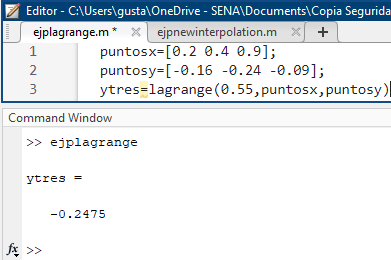
\includegraphics[width=0.6\textwidth]{30a.png}
    \caption{Confirmación B}
    \label{fig:imagen1}
    \end{figure}
    \newpage
\begin{itemize}
    \item 31.  Given the data in the following table:
          \newline a. Interpolate at x = 3 with a first-degree Lagrange polynomial
          using two most suitable data points.
          \newline b. Interpolate at x = 3 with a second-degree Lagrange polynomial
          using three most suitable data points.
          \newline c. Compare the results of (a) and (b), and discuss.
\end{itemize}

\begin{table}[h!]
    \begin{tabular}{l|l|l|l|l}
        \hline
        \multicolumn{1}{|p{30.865313pt}}{\raggedright x} & \multicolumn{1}{|p{30.865313pt}}{\raggedright 0} & \multicolumn{1}{|p{30.865313pt}}{\raggedright 1}    & \multicolumn{1}{|p{30.1125pt}}{\raggedright 2}    & \multicolumn{1}{|p{30.1125pt}|}{\raggedright 4}    \\
        \cline{1-5}
        \multicolumn{1}{|p{30.865313pt}}{\raggedright y} & \multicolumn{1}{|p{30.865313pt}}{\raggedright 1} & \multicolumn{1}{|p{30.865313pt}}{\raggedright 0.96} & \multicolumn{1}{|p{30.1125pt}}{\raggedright 1.68} & \multicolumn{1}{|p{30.1125pt}|}{\raggedright 1.82} \\
        \hline
    \end{tabular}
\end{table}

a)
\begin{equation*}
    L(x) = \frac{42}{25}\frac{(x-4)}{(2-4)}+\frac{91}{50}\frac{(x-2)}{(4-2)}  
\end{equation*}
\begin{equation*}
    L(x) = \frac{7}{100}x+\frac{77}{50}
\end{equation*}
\begin{equation*}
    L(x) = \frac{7}{100}(3)+\frac{77}{50}=\boxed{1.75}
\end{equation*}
b)
\begin{equation*}
    L(x) = \frac{24}{25}\frac{(x-2) \cdot (x-4)}{(1-2) \cdot (1-4)}+\frac{42}{25}\frac{(x-1) \cdot (x-4)}{(2-1) \cdot (2-4)}+\frac{91}{50}\frac{(x-1) \cdot (x-2)}{(4-1) \cdot (4-2)}    
\end{equation*}
\begin{equation*}
    L(x) = -\frac{13}{60}x^2+\frac{137}{100}x-\frac{29}{150}
\end{equation*}
\begin{equation*}
    L(x) = -\frac{13}{60}(3)^2+\frac{137}{100}(3)-\frac{29}{150}=\boxed{1.9666}
\end{equation*}
c) La estimación proporcionada en b) es claramente superior porque los datos se utilizaron de manera más efectiva para la interpolación. Se acerca más al valor del polinomio de tercer grado \boxed{2.265} 
\newpage
\begin{itemize}
    \item 32. Given the data in the following table:
          \newline a. Interpolate at x = 2.5 with a first-degree Lagrange polynomial
          using two most suitable data points.
          \newline b. Interpolate at x = 2.5 with a second-degree Lagrange polynomial
          using three most suitable data points.
          \newline c. Compare the results of (a) and (b), and discuss.
\end{itemize}

\begin{table}[h!]
    \begin{tabular}{|l|l|l|l|l|l|}
        \hline
        \multicolumn{1}{|p{30.865313pt}}{\raggedright x} & \multicolumn{1}{|p{30.865313pt}}{\raggedright 1} & \multicolumn{1}{|p{33.12375pt}}{\raggedright 1.5}    & \multicolumn{1}{|p{33.876564pt}}{\raggedright 2}      & \multicolumn{1}{|p{33.876564pt}}{\raggedright 3}      & \multicolumn{1}{|p{33.876564pt}|}{\raggedright 5}      \\
        \cline{1-6}
        \multicolumn{1}{|p{30.865313pt}}{\raggedright y} & \multicolumn{1}{|p{30.865313pt}}{\raggedright 0} & \multicolumn{1}{|p{33.12375pt}}{\raggedright 0.1761} & \multicolumn{1}{|p{33.876564pt}}{\raggedright 0.3010} & \multicolumn{1}{|p{33.876564pt}}{\raggedright 0.4771} & \multicolumn{1}{|p{33.876564pt}|}{\raggedright 0.6990} \\
        \hline
    \end{tabular}
\end{table}

a)
\begin{equation*}
    L(x) = \frac{301}{1000}\frac{(x-3)}{(2-3)}+\frac{4771}{10000}\frac{(x-2)}{(3-2)}   
\end{equation*}
\begin{equation*}
    L(x) = \frac{1761}{10000}x-\frac{32}{625}    
\end{equation*}
\begin{equation*}
    L(x) = \frac{1761}{10000}(2.5)-\frac{32}{625}=\boxed{0.38905}   
\end{equation*}
b)
\begin{equation*}
    L(x) = \frac{1761}{10000}\frac{(x-2) \cdot (x-3)}{(\frac{3}{2}-2) \cdot (\frac{3}{2}-3)}+\frac{301}{1000}\frac{(x-\frac{3}{2}) \cdot (x-3)}{(2-\frac{3}{2}) \cdot (2-3)}+\frac{4771}{10000}\frac{(x-\frac{3}{2}) \cdot (x-2)}{(3-\frac{3}{2}) \cdot (3-2)}    
\end{equation*}
\begin{equation*}
    L(x) = -\frac{737}{15000}x^2+\frac{12653}{30000}x-\frac{173}{500}    
\end{equation*}
\begin{equation*}
    L(x) = -\frac{737}{15000}(2.5)^2+\frac{12653}{30000}(2.5)-\frac{173}{500}=\boxed{0.401333}
\end{equation*}
c) La estimación proporcionada en b) es claramente superior porque los datos se utilizaron de manera más efectiva para la interpolación. Se acerca más al valor del polinomio de cuarto grado \boxed{0.3964375}
\newpage
\begin{itemize}
    \item 33. Using format long and the user-defined function Lagrange
          Interp, given the data in the following table:
          \newline a. Interpolate at x = 0.6 with a second-degree Lagrange polynomial
          using three most suitable data points.
          \newline  b. Interpolate at x = 0.6 with a third-degree Lagrange polynomial
          using four most suitable data points.
          \newline c. Compare the results of (a) and (b).
\end{itemize}

\begin{table}[h!]
    \begin{tabular}{lllllll}
        \hline
        \multicolumn{1}{|p{30.865313pt}}{\raggedright x} & \multicolumn{1}{|p{33.12375pt}}{\raggedright 0.2}    & \multicolumn{1}{|p{39.899063pt}|}{\raggedright 0.4}   & \multicolumn{1}{|p{33.876564pt}|}{\raggedright 0.5}   & \multicolumn{1}{|p{33.876564pt}|}{\raggedright 0.8}   & \multicolumn{1}{|p{33.876564pt}|}{\raggedright 1.1}   & \multicolumn{1}{|p{33.876564pt}|}{\raggedright 1.3}    \\
        \hline
        \multicolumn{1}{|p{30.865313pt}}{\raggedright y} & \multicolumn{1}{|p{33.12375pt}}{\raggedright 0.9048} & \multicolumn{1}{|p{39.899063pt}}{\raggedright 0.8187} & \multicolumn{1}{|p{33.876564pt}}{\raggedright 0.7788} & \multicolumn{1}{|p{33.876564pt}}{\raggedright 0.6703} & \multicolumn{1}{|p{33.876564pt}}{\raggedright 0.5769} & \multicolumn{1}{|p{33.876564pt}|}{\raggedright 0.5220} \\
        \hline
    \end{tabular}
\end{table}
a)
\begin{figure}[H]
    \centering
    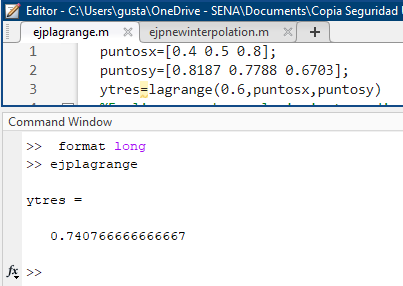
\includegraphics[width=0.6\textwidth]{33a.png}
    \caption{Polinomio segundo grado}
    \label{fig:imagen1}
    \end{figure}
\newpage
b)
    \begin{figure}[H]
        \centering
        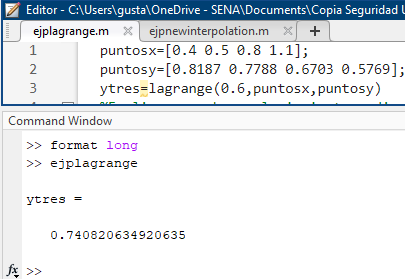
\includegraphics[width=0.5\textwidth]{33b.png}
        \caption{Polinomio tercer grado}
        \label{fig:imagen1}
        \end{figure}
c) La estimación proporcionada en b) es claramente superior porque los datos se utilizaron de manera más efectiva para la interpolación. Se acerca más al valor de quinto grado \boxed{0.740829629629630}
\begin{figure}[H]
    \centering
    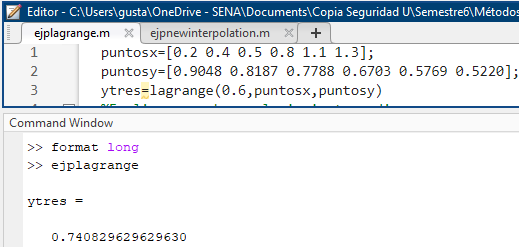
\includegraphics[width=0.5\textwidth]{33c.png}
    \caption{Polinomio quinto grado}
    \label{fig:imagen1}
    \end{figure}
\begin{itemize}
    \item 34. Using format long and the user-defined function Lagrange
          Interp, given the data in the following table:
          \newline  a. Interpolate at x = 0.6 with a second-degree Lagrange polynomial
          using three most suitable data points.
          \newline  b. Interpolate at x = 0.6 with a third-degree Lagrange polynomial
          using four most suitable data points.
          \newline  c. Compare the results of (a) and (b).
\end{itemize}

\begin{table}[h!]
    \begin{tabular}{l|l|l|l|l|l|l}
        \hline
        \multicolumn{1}{|p{30.865313pt}}{\raggedright x} & \multicolumn{1}{|p{31.618126pt}}{\raggedright 0.1}    & \multicolumn{1}{|p{31.618126pt}}{\raggedright 0.2}    & \multicolumn{1}{|p{33.876564pt}}{\raggedright 0.4}    & \multicolumn{1}{|p{37.640625pt}}{\raggedright 0.7}    & \multicolumn{1}{|p{33.876564pt}}{\raggedright 0.9}    & \multicolumn{1}{|p{33.876564pt}|}{\raggedright 1.0}    \\
        \hline
        \multicolumn{1}{|p{30.865313pt}}{\raggedright y} & \multicolumn{1}{|p{31.618126pt}}{\raggedright 0.9330} & \multicolumn{1}{|p{31.618126pt}}{\raggedright 0.8706} & \multicolumn{1}{|p{33.876564pt}}{\raggedright 0.7579} & \multicolumn{1}{|p{37.640625pt}}{\raggedright 0.6156} & \multicolumn{1}{|p{33.876564pt}}{\raggedright 0.5359} & \multicolumn{1}{|p{33.876564pt}|}{\raggedright 0.5000} \\
        \hline
    \end{tabular}
\end{table}

a)
\begin{figure}[H]
    \centering
    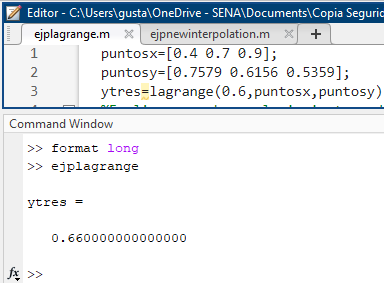
\includegraphics[width=0.6\textwidth]{34a.png}
    \caption[short]{Polinomio segundo grado}
\end{figure}
b)
\begin{figure}[H]
    \centering
    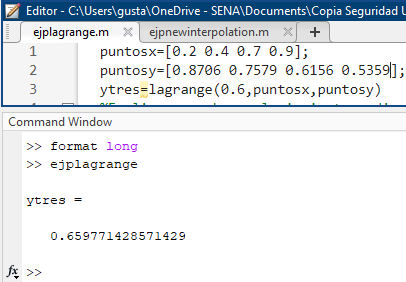
\includegraphics[width=0.6\textwidth]{34b.png}
    \caption[short]{Polinomio tercer grado}
\end{figure}
c) La estimación proporcionada en b) es claramente superior porque los datos se utilizaron de manera más efectiva para la interpolación. Se acerca más al valor de quinto grado \boxed{0.659780423280423}
\begin{figure}[H]
    \centering
    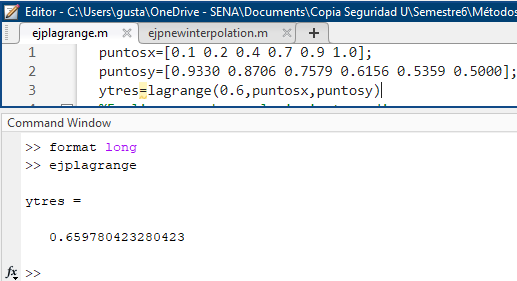
\includegraphics[width=0.63\textwidth]{34c.png}
    \caption[short]{Polinomio quinto grado}
\end{figure}
\newpage 
\begin{itemize}
    \item 35. Using the user-defined function LagrangeInterp, given the
          data in the following table:
          \newline   a. Interpolate at x = 1.7 with a second-degree Lagrange polynomial
          using three most suitable data points.
          \newline b. Interpolate at x = 9 with a third-degree Lagrange polynomial
          using four most suitable data points.
\end{itemize}

\begin{table}[h!]
    \begin{tabular}{l|l|l|l|l|l}
        \hline    
        \multicolumn{1}{|p{30.865313pt}}{\raggedright x} & \multicolumn{1}{|p{31.618126pt}}{\raggedright 0} & \multicolumn{1}{|p{31.618126pt}}{\raggedright 1} & \multicolumn{1}{|p{33.876564pt}}{\raggedright 3}    & \multicolumn{1}{|p{37.640625pt}}{\raggedright 7}    & \multicolumn{1}{|p{33.876564pt}|}{\raggedright 12}   \\
        \hline
        \multicolumn{1}{|p{30.865313pt}}{\raggedright y} & \multicolumn{1}{|p{31.618126pt}}{\raggedright 0} & \multicolumn{1}{|p{31.618126pt}}{\raggedright 1} & \multicolumn{1}{|p{33.876564pt}}{\raggedright 1.44} & \multicolumn{1}{|p{37.640625pt}}{\raggedright 1.91} & \multicolumn{1}{|p{33.876564pt}|}{\raggedright 2.29} \\
        \hline
    \end{tabular}
\end{table}
a)
\begin{figure}[H]
    \centering
    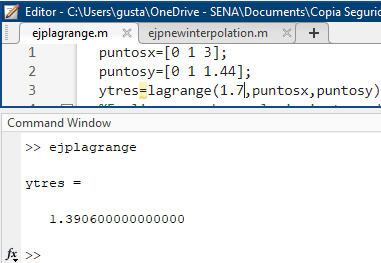
\includegraphics[width=0.55\textwidth]{35a.png}
    \caption[short]{Polinomio segundo grado}
\end{figure}
b)
\begin{figure}[H]
    \centering
    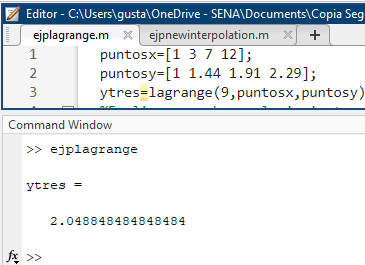
\includegraphics[width=0.55\textwidth]{35b.png}
    \caption[short]{Polinomio tercer grado}
\end{figure}
\begin{itemize}
    \item 36. Using the user-defined function LagrangeInterp, given the
          data in the following table:
          \newline  a. Interpolate at x = 1.5 with a second-degree Lagrange polynomial
          using three most suitable data points.
          \newline  b. Interpolate at x = 3 with a third-degree Lagrange polynomial
          using four most suitable data points.
\end{itemize}\begin{table}[h!]
    \begin{tabular}{|l|l|l|l|l|l|}
        \hline
        \multicolumn{1}{|p{30.865313pt}}{\raggedright x} & \multicolumn{1}{|p{31.618126pt}}{\raggedright 0} & \multicolumn{1}{|p{31.618126pt}}{\raggedright 1} & \multicolumn{1}{|p{33.876564pt}}{\raggedright 2}   & \multicolumn{1}{|p{37.640625pt}}{\raggedright 2.5}  & \multicolumn{1}{|p{33.876564pt}|}{\raggedright 4}    \\
        \hline
        \multicolumn{1}{|p{30.865313pt}}{\raggedright y} & \multicolumn{1}{|p{31.618126pt}}{\raggedright 1} & \multicolumn{1}{|p{31.618126pt}}{\raggedright 1} & \multicolumn{1}{|p{33.876564pt}}{\raggedright 0.6} & \multicolumn{1}{|p{37.640625pt}}{\raggedright 0.48} & \multicolumn{1}{|p{33.876564pt}|}{\raggedright 0.29} \\
        \hline
    \end{tabular}
\end{table}
a)
\begin{figure}[H]
    \centering
    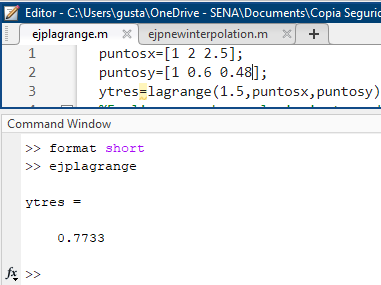
\includegraphics[width=0.5\textwidth]{36a.png}
    \caption[short]{Polinomio segundo grado}
\end{figure}
b)
\begin{figure}[H]
    \centering
    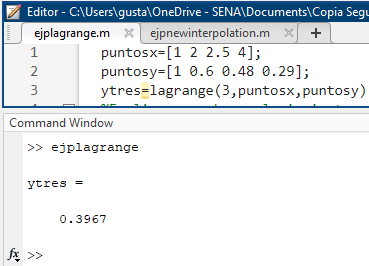
\includegraphics[width=0.5\textwidth]{36b.png}
    \caption[short]{Polinomio tercer grado}
\end{figure}

\newpage
\begin{itemize}
    \item 37. For the data in the following table, construct a divided differences
          table and interpolate at x = 0.25 using Newton interpolating
          polynomials p1(x), p2(x), and p3(x).
\end{itemize}

\begin{table}[h!]
    \begin{tabular}{l|l|l|l|l}
        \hline
        \multicolumn{1}{|p{30.865313pt}}{\raggedright x} & \multicolumn{1}{|p{31.618126pt}}{\raggedright 0} & \multicolumn{1}{|p{33.12375pt}}{\raggedright 0.5}    & \multicolumn{1}{|p{33.876564pt}}{\raggedright 0.9}    & \multicolumn{1}{|p{37.640625pt}|}{\raggedright 1.2}    \\
        \hline
        \multicolumn{1}{|p{30.865313pt}}{\raggedright y} & \multicolumn{1}{|p{31.618126pt}}{\raggedright 1} & \multicolumn{1}{|p{33.12375pt}}{\raggedright 0.9098} & \multicolumn{1}{|p{33.876564pt}}{\raggedright 0.7725} & \multicolumn{1}{|p{37.640625pt}|}{\raggedright 0.6626} \\
        \hline
    \end{tabular}
\end{table}
Para los puntos las diferencias divididas quedan de la forma:

\begin{center}
    \begin{tabular}{|c|c|c|c|c|c|}
    \hline
    \textbf{$j$} & \textbf{$X$} & \textbf{1st Divided Diff} & \textbf{2nd Divided Diff} & \textbf{3rd Divided Diff} & \textbf{4th Divided Diff} \\
    \hline
    0 & 0 & 1 & xxxxxxxxxxx & xxxxxxxxxxx & xxxxxxxxxxx\\
    \hline
    1 & 0.5 & 0.9098 & -0.1804 & xxxxxxxxxxx & xxxxxxxxxxx \\
    \hline
    2 & 0.9 & 0.7726 & -0.3430 & -1.3085 & xxxxxxxxxxx \\
    \hline
    3 & 1.2 & 0.6626 & -0.6667 & -1.0767 & -7.9507 \\
    \hline
    \end{tabular}
    \end{center}    

\begin{equation*}
    \displaystyle{P_1(x) = 1+\left(\frac{1}{0-\frac{1}{2}}+\frac{\frac{4549}{5000}}{\frac{1}{2}-0}\right)\left(x-0\right)}
\end{equation*}
\begin{equation*}
    P_1(x) =  -\frac{451}{2500}x+1
\end{equation*}
\begin{equation*}
    P_1(0.25) =  -\frac{451}{2500}(0.25)+1=\boxed{0.9549}
\end{equation*}
\begin{equation*}
    \displaystyle{P_2(x) = 1+\left(\frac{1}{0-\frac{1}{2}}+\frac{\frac{4549}{5000}}{\frac{1}{2}-0}\right)\left(x-0\right)+\left(\frac{1}{\left(0-\frac{1}{2}\right)\left(0-\frac{9}{10}\right)}+\frac{\frac{4549}{5000}}{\left(\frac{1}{2}-0\right)\left(\frac{1}{2}-\frac{9}{10}\right)}+\frac{\frac{309}{400}}{\left(\frac{9}{10}-0\right)\left(\frac{9}{10}-\frac{1}{2}\right)}\right)\left(\left(x-0\right)\left(x-\frac{1}{2}\right)\right)}    
\end{equation*}
\begin{equation*}
    P_2(x) =-\frac{3257}{18000}x^{2}-\frac{16187}{180000}x+1
\end{equation*}
\begin{equation*}
    P_2(0.25) =-\frac{3257}{18000}(0.25)^{2}-\frac{16187}{180000}(0.25)+1=\boxed{0.9662090277777778}
\end{equation*}
\begin{equation*}
    \displaystyle{P_3(x) = 1+\left(\frac{1}{0-\frac{1}{2}}+\frac{\frac{4549}{5000}}{\frac{1}{2}-0}\right)\left(x-0\right)+\left(\frac{1}{\left(0-\frac{1}{2}\right)\left(0-\frac{9}{10}\right)}+\frac{\frac{4549}{5000}}{\left(\frac{1}{2}-0\right)\left(\frac{1}{2}-\frac{9}{10}\right)}+\frac{\frac{309}{400}}{\left(\frac{9}{10}-0\right)\left(\frac{9}{10}-\frac{1}{2}\right)}\right)}
    \end{equation*}
\begin{equation*}
    \left(\left(x-0\right)\left(x-\frac{1}{2}\right)\right)+\left(\frac{1}{\left(\left(0-\frac{1}{2}\right)\left(0-\frac{9}{10}\right)\right)\left(0-\frac{6}{5}\right)}+\frac{\frac{4549}{5000}}{\left(\left(\frac{1}{2}-0\right)\left(\frac{1}{2}-\frac{9}{10}\right)\right)\left(\frac{1}{2}-\frac{6}{5}\right)}+\frac{\frac{309}{400}}{\left(\left(\frac{9}{10}-0\right)\left(\frac{9}{10}-\frac{1}{2}\right)\right)\left(\frac{9}{10}-\frac{6}{5}\right)}\right)
\end{equation*}
\begin{equation*}
    +\frac{\frac{3313}{5000}}{\left(\left(\frac{6}{5}-0\right)\left(\frac{6}{5}-\frac{1}{2}\right)\right)\left(\frac{6}{5}-\frac{9}{10}\right)}\left(\left(\left(x-0\right)\left(x-\frac{1}{2}\right)\right)\left(x-\frac{9}{10}\right)\right)
\end{equation*}
\begin{equation*}
    P_3(x) =\frac{4661}{37800}x^{3}-\frac{19093}{54000}x^{2}-\frac{21697}{630000}x+1
\end{equation*}
\begin{equation*}
    P_3(0.25) =\frac{4661}{37800}(0.25)^{3}-\frac{19093}{54000}(0.25)^{2}-\frac{21697}{630000}(0.25)+1= \boxed{0.9712183697089947}
\end{equation*}

\begin{figure}[H]
    \centering
    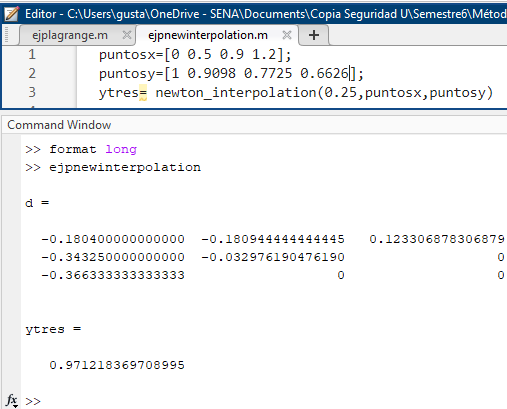
\includegraphics[width=0.6\textwidth]{37a.png}
    \caption{Confirmación con NewtonInterp}
\end{figure}
\newpage
\begin{itemize}
    \item 38. For the data in the following table, construct a divided differences
          table and interpolate at x = 0.3 using Newton interpolating
          polynomials p1(x), p2(x), and p3(x).
\end{itemize}

\begin{table}[h!]
    \begin{tabular}{|lllll|}
        \hline
        \multicolumn{1}{|p{30.865313pt}}{\raggedright x} & \multicolumn{1}{|p{30.865313pt}}{\raggedright 0} & \multicolumn{1}{|p{32.370937pt}}{\raggedright 0.4}  & \multicolumn{1}{|p{30.1125pt}}{\raggedright 0.8}  & \multicolumn{1}{|p{30.1125pt}|}{\raggedright 1}    \\
        \hline
        \multicolumn{1}{|p{30.865313pt}}{\raggedright y} & \multicolumn{1}{|p{30.865313pt}}{\raggedright 1} & \multicolumn{1}{|p{32.370937pt}}{\raggedright 2.68} & \multicolumn{1}{|p{30.1125pt}}{\raggedright 5.79} & \multicolumn{1}{|p{30.1125pt}|}{\raggedright 8.15} \\
        \hline
    \end{tabular}
\end{table}
Para los puntos las diferencias divididas quedan de la forma:
\begin{center}
    \begin{tabular}{|c|c|c|c|c|c|}
    \hline
    \textbf{$j$} & \textbf{$X$} & \textbf{1st Divided Diff} & \textbf{2nd Divided Diff} & \textbf{3rd Divided Diff} & \textbf{4th Divided Diff} \\
    \hline
    0 & 0 & 1 & xxxxxxxxxxx & xxxxxxxxxxx & xxxxxxxxxxx\\
    \hline
    1 & 0.4 & 2.68 & 4.2000 & xxxxxxxxxxx & xxxxxxxxxxx \\
    \hline
    2 & 0.8 & 5.79 & 7.7750 & 8.9375 & xxxxxxxxxxx \\
    \hline
    3 & 1 & 8.75 & 14.8000 & 35.1250 & 130.9375 \\
    \hline
    \end{tabular}
    \end{center}
\begin{equation*}
    \displaystyle{P_1(x) = 1+\left(\frac{1}{0-\frac{2}{5}}+\frac{\frac{67}{25}}{\frac{2}{5}-0}\right)\left(x-0\right)}    
\end{equation*}
\begin{equation*}
    P_1(x) =  \frac{21}{5}x+1
\end{equation*}
\begin{equation*}
    P_1(0.3) =  \frac{21}{5}(0.3)+1=\boxed{2.26}
\end{equation*}
\begin{equation*}
    \displaystyle{P_2(x) = 1+\left(\frac{1}{0-\frac{2}{5}}+\frac{\frac{67}{25}}{\frac{2}{5}-0}\right)\left(x-0\right)+\left(\frac{1}{\left(0-\frac{2}{5}\right)\left(0-\frac{4}{5}\right)}+\frac{\frac{67}{25}}{\left(\frac{2}{5}-0\right)\left(\frac{2}{5}-\frac{4}{5}\right)}+\frac{\frac{579}{100}}{\left(\frac{4}{5}-0\right)\left(\frac{4}{5}-\frac{2}{5}\right)}\right)\left(\left(x-0\right)\left(x-\frac{2}{5}\right)\right)}    
\end{equation*}
\begin{equation*}
    P_2(x) =\frac{143}{32}x^{2}+\frac{193}{80}x+1
\end{equation*}
\begin{equation*}
    P_2(0.3) =\frac{143}{32}(0.3)^{2}+\frac{193}{80}(0.3)+1=\boxed{2.1259375}
\end{equation*}
\begin{equation*}
    \displaystyle{P_3(x) = 1+\left(\frac{1}{0-\frac{2}{5}}+\frac{\frac{67}{25}}{\frac{2}{5}-0}\right)\left(x-0\right)+\left(\frac{1}{\left(0-\frac{2}{5}\right)\left(0-\frac{4}{5}\right)}+\frac{\frac{67}{25}}{\left(\frac{2}{5}-0\right)\left(\frac{2}{5}-\frac{4}{5}\right)}+\frac{\frac{579}{100}}{\left(\frac{4}{5}-0\right)\left(\frac{4}{5}-\frac{2}{5}\right)}\right)\left(\left(x-0\right)\left(x-\frac{2}{5}\right)\right)}
\end{equation*}
\begin{equation*}
    +\left(\frac{1}{\left(\left(0-\frac{2}{5}\right)\left(0-\frac{4}{5}\right)\right)\left(0-1\right)}+\frac{\frac{67}{25}}{\left(\left(\frac{2}{5}-0\right)\left(\frac{2}{5}-\frac{4}{5}\right)\right)\left(\frac{2}{5}-1\right)}+\frac{\frac{579}{100}}{\left(\left(\frac{4}{5}-0\right)\left(\frac{4}{5}-\frac{2}{5}\right)\right)\left(\frac{4}{5}-1\right)}+\frac{\frac{163}{20}}{\left(\left(1-0\right)\left(1-\frac{2}{5}\right)\right)\left(1-\frac{4}{5}\right)}\right)    
\end{equation*}
$$\left(\left(\left(x-0\right)\left(x-\frac{2}{5}\right)\right)\left(x-\frac{4}{5}\right)\right)$$
\begin{equation*}
    P_3(x) =\frac{215}{96}x^{3}+\frac{57}{32}x^{2}+\frac{751}{240}x+1
\end{equation*}
\begin{equation*}
    P_3(0.3) =\frac{215}{96}(0.3)^{3}+\frac{57}{32}(0.3)^{2}+\frac{751}{240}x+1= \boxed{2.15953125}
\end{equation*}

\begin{figure}[H]
    \centering
    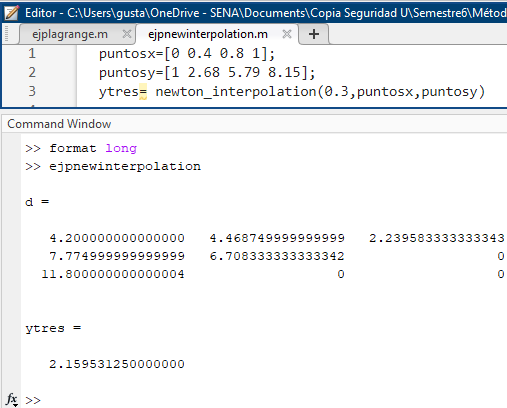
\includegraphics[width=0.6\textwidth]{38.png}
    \caption{Confirmación con NewtonInterp}
\end{figure}


\begin{itemize}
    \item 39. Consider the data in the following table.
          \newline  a. Construct a divided differences table and interpolate at x = 1.75
          using the third-degree Newton interpolating polynomial p3(x).
          \newline  b. Suppose one more point (x = 3, y = 9.11) is added to the data.
          Update the divided-differences table from (a) and interpolate at
          x = 1.75 using the fourth-degree Newton interpolating polynomial
          p4(x).
\end{itemize}

\begin{table}[h!]
    \begin{tabular}{l|l|l|l|l}
        \hline
        \multicolumn{1}{|p{30.865313pt}}{\raggedright x} & \multicolumn{1}{|p{30.865313pt}}{\raggedright 1}    & \multicolumn{1}{|p{32.370937pt}}{\raggedright 1.5}  & \multicolumn{1}{|p{30.1125pt}}{\raggedright 2}    & \multicolumn{1}{|p{30.1125pt}|}{\raggedright 2.5}  \\
        \hline
        \multicolumn{1}{|p{30.865313pt}}{\raggedright y} & \multicolumn{1}{|p{30.865313pt}}{\raggedright 1.22} & \multicolumn{1}{|p{32.370937pt}}{\raggedright 2.69} & \multicolumn{1}{|p{30.1125pt}}{\raggedright 4.48} & \multicolumn{1}{|p{30.1125pt}|}{\raggedright 6.59} \\
        \hline
    \end{tabular}
\end{table}

\begin{itemize}
    \item 40. Consider the data in the following table.
          \newline  a. Construct a divided differences table and interpolate at x = 4
          using the third-degree Newton interpolating polynomial p3(x).
          \newline  b. Suppose one more point (x = 7, y = 0.18) is added to the data.
          Update the divided-difference table from (a) and interpolate at
          x = 4 using the fourth-degree Newton interpolating polynomial
          p4(x).
\end{itemize}

\begin{table}[h!]
    \begin{tabular}{l|l|l|l|l}
        \hline
        \multicolumn{1}{|p{30.865313pt}}{\raggedright x} & \multicolumn{1}{|p{30.865313pt}}{\raggedright 1} & \multicolumn{1}{|p{32.370937pt}}{\raggedright 3}    & \multicolumn{1}{|p{30.1125pt}}{\raggedright 5}    & \multicolumn{1}{|p{30.1125pt}|}{\raggedright 6}    \\
        \hline
        \multicolumn{1}{|p{30.865313pt}}{\raggedright y} & \multicolumn{1}{|p{30.865313pt}}{\raggedright 1} & \multicolumn{1}{|p{32.370937pt}}{\raggedright 0.45} & \multicolumn{1}{|p{30.1125pt}}{\raggedright 0.26} & \multicolumn{1}{|p{30.1125pt}|}{\raggedright 0.21} \\
        \hline
    \end{tabular}
\end{table}
\newpage
\begin{itemize}
    \item 41. Given the data in the following table
          \newline  a. Construct a divided differences table and interpolate at x = 2.4
          and x = 4.2 using the fourth-degree Newton interpolating polynomial
          p4(x).    
          \newline   b. Confirm the results by executing the user-defined function
          NewtonInterp.
\end{itemize}

\begin{table}[h!]
    \begin{tabular}{l|l|l|l|l|l}
        \hline
        \multicolumn{1}{|p{30.865313pt}}{\raggedright x} & \multicolumn{1}{|p{30.865313pt}}{\raggedright 1}    & \multicolumn{1}{|p{32.370937pt}}{\raggedright 2}    & \multicolumn{1}{|p{30.1125pt}}{\raggedright 3}    & \multicolumn{1}{|p{30.1125pt}}{\raggedright 4}    & \multicolumn{1}{|p{30.1125pt}|}{\raggedright 6}    \\
        \hline
        \multicolumn{1}{|p{30.865313pt}}{\raggedright y} & \multicolumn{1}{|p{30.865313pt}}{\raggedright 0.69} & \multicolumn{1}{|p{32.370937pt}}{\raggedright 1.10} & \multicolumn{1}{|p{30.1125pt}}{\raggedright 1.39} & \multicolumn{1}{|p{30.1125pt}}{\raggedright 1.61} & \multicolumn{1}{|p{30.1125pt}|}{\raggedright 1.95} \\
        \hline
    \end{tabular}
\end{table}

\begin{itemize}
    \item 42. Given the data in the following table
          \newline   a. Construct a divided differences table and interpolate at x = 2.5
          and x = 5 using the fourth-degree Newton interpolating polynomial
          p4(x).
          \newline   b. Confirm the results by executing the user-defined function
          NewtonInterp.
\end{itemize}

\begin{table}[h!]
    \begin{tabular}{llllll}
        \hline
        \multicolumn{1}{|p{30.865313pt}}{\raggedright x} & \multicolumn{1}{|p{30.865313pt}}{\raggedright 1}    & \multicolumn{1}{|p{32.370937pt}}{\raggedright 2}    & \multicolumn{1}{|p{30.1125pt}}{\raggedright 3}    & \multicolumn{1}{|p{30.1125pt}}{\raggedright 4}    & \multicolumn{1}{|p{30.1125pt}|}{\raggedright 6}    \\
        \hline
        \multicolumn{1}{|p{30.865313pt}}{\raggedright y} & \multicolumn{1}{|p{30.865313pt}}{\raggedright 0.89} & \multicolumn{1}{|p{32.370937pt}}{\raggedright 1.81} & \multicolumn{1}{|p{30.1125pt}}{\raggedright 2.94} & \multicolumn{1}{|p{30.1125pt}}{\raggedright 4.38} & \multicolumn{1}{|p{30.1125pt}|}{\raggedright 8.72} \\
        \hline
    \end{tabular}
\end{table}

\begin{itemize}
    \item 43. Using the user-defined function NewtonInterp, given the data
          in the following table, interpolate at x = 4.5 via Newton interpolating
          polynomials of all possible degrees, and comment on accuracy.
\end{itemize}

\begin{table}[h!]
    \begin{tabular}{l|l|l|l|l|l|l|l}
        \hline
        \multicolumn{1}{|p{30.865313pt}}{\raggedright x} & \multicolumn{1}{|p{30.865313pt}}{\raggedright 1} & \multicolumn{1}{|p{32.370937pt}}{\raggedright 2}      & \multicolumn{1}{|p{33.876564pt}}{\raggedright 3.5}    & \multicolumn{1}{|p{37.640625pt}}{\raggedright 5}      & \multicolumn{1}{|p{33.876564pt}}{\raggedright 7}      & \multicolumn{1}{|p{30.1125pt}}{\raggedright 9} & \multicolumn{1}{|p{33.876564pt}|}{\raggedright 10}     \\
        \hline
        \multicolumn{1}{|p{30.865313pt}}{\raggedright y} & \multicolumn{1}{|p{30.865313pt}}{\raggedright 1} & \multicolumn{1}{|p{32.370937pt}}{\raggedright 1.4142} & \multicolumn{1}{|p{33.876564pt}}{\raggedright 1.8708} & \multicolumn{1}{|p{37.640625pt}}{\raggedright 2.2361} & \multicolumn{1}{|p{33.876564pt}}{\raggedright 2.6458} & \multicolumn{1}{|p{30.1125pt}}{\raggedright 3} & \multicolumn{1}{|p{33.876564pt}|}{\raggedright 3.1623} \\
        \hline
    \end{tabular}
\end{table}

\end{document}